\documentclass[aspectratio=169]{beamer}
\usetheme[titleformat=regular, sectionpage=progressbar, progressbar=head, background=light, numbering=none]{metropolis}           % Use metropolis theme

\usepackage{multicol}
\usepackage[utf8]{inputenc}
\usepackage[T1]{fontenc}
\usepackage{bytefield}
\usepackage{subcaption}
\captionsetup{format=hang}
\usepackage{pgf-umlsd}
\usepackage{pgf-umlcd}
\usepackage[spanish]{babel}
\usepackage[style=ieee, sorting=none]{biblatex}
\usepackage{csquotes}
\usepackage{listings}
\usepackage{sourcecodepro}
\usepackage{tikz}
\usetikzlibrary{shapes.geometric, arrows}
\usepackage{tikz-qtree}
\usepackage[labelfont=bf]{caption}
\usepackage{hyperref}
\usepackage[htt]{hyphenat}
\usepackage{booktabs}
\usepackage{pgfplots}
\usetikzlibrary{plotmarks}
\usepgfplotslibrary{groupplots}
\pgfplotsset{compat=newest}
\usepackage[sfdefault]{roboto}
\usepackage{multirow}
\usepackage{textcomp}

\newlength\figureheight
\newlength\figurewidth
\setlength\figureheight{9cm}
\setlength\figurewidth{\linewidth}

% CPP style definition: %
\renewcommand{\lstlistingname}{Código}% Listing -> Código
\renewcommand{\lstlistlistingname}{Lista de \lstlistingname s}% List of Listings -> List of Algorithms
\definecolor{dkgreen}{rgb}{0,0.6,0}
\definecolor{gray}{rgb}{0.5,0.5,0.5}
\definecolor{lightgray}{rgb}{0.95, 0.95, 0.95}
\definecolor{mauve}{rgb}{0.58,0,0.82}
\definecolor{mygreen}{rgb}{0,0.6,0}
\definecolor{mygray}{rgb}{0.5,0.5,0.5}
\definecolor{mymauve}{rgb}{0.58,0,0.82}
\lstdefinestyle{CPP}{ % Estilo de lenguaje C++11
    language=[11]C++,
    frame=Lbtr,
    xleftmargin=\parindent,
    captionpos=b,
    aboveskip=3mm,
    belowskip=3mm,
    showstringspaces=false,
    columns=flexible,
    basicstyle={\small\ttfamily},
    numbers=left,
    numberstyle=\tiny\color{gray},
    keywordstyle=\color{purple},
    commentstyle=\color{gray},
    stringstyle=\color{dkgreen},
    breaklines=true,
    breakatwhitespace=true,
    tabsize=4,
    morekeywords={string,define,\#},
    otherkeywords={\#},
    backgroundcolor=\color{lightgray},
    escapeinside={/l*}{*l/}
}

\lstdefinestyle{myXML}{ % Estilo de lenguaje C++11
    language=XML,
    frame=Lbtr,
    xleftmargin=\parindent,
    captionpos=b,
    aboveskip=3mm,
    belowskip=3mm,
    showstringspaces=false,
    columns=flexible,
    basicstyle={\small\ttfamily},
    numbers=left,
    numberstyle=\tiny\color{gray},
    keywordstyle=\color{purple},
    commentstyle=\color{gray},
    stringstyle=\color{dkgreen},
    breaklines=true,
    breakatwhitespace=true,
    tabsize=4,
    morekeywords={xml,version, launch, basedir, network, seed},
    otherkeywords={\#},
    backgroundcolor=\color{lightgray},
    escapeinside={/l*}{*l/}
}

\lstdefinestyle{MyPython}{ % Estilo de lenguaje C++11
    language=Python,
    frame=Lbtr,
    xleftmargin=\parindent,
    captionpos=b,
    aboveskip=3mm,
    belowskip=3mm,
    showstringspaces=false,
    columns=flexible,
    basicstyle={\small\ttfamily},
    numbers=left,
    numberstyle=\tiny\color{gray},
    keywordstyle=\color{purple},
    commentstyle=\color{gray},
    stringstyle=\color{dkgreen},
    breaklines=true,
    breakatwhitespace=true,
    tabsize=4,
    morekeywords={traci, print},
    otherkeywords={},
    backgroundcolor=\color{lightgray},
    escapeinside={/l*}{*l/}
}

% new an instance thread
% Example:
% \newthread[edge distance]{var}{thread name}
\renewcommand{\newthread}[3][0.2]{
    \newinst[#1]{#2}{#3}
    \stepcounter{threadnum}
    \node[below of=inst\theinstnum,node distance=0.8cm] (thread\thethreadnum) {};
    \tikzstyle{threadcolor\thethreadnum}=[fill=gray!30]
    \tikzstyle{instcolor#2}=[fill=gray!30]
}

\addbibresource{bibliografia.bib}



\title{Diseño e Implementación de un Framework Integrado para la Simulación de Sistemas Inteligentes de Transporte en OMNeT++ y Paramics}
\date{\today}
\author{Manuel Olguín \\\href{mailto:molguin@dcc.uchile.cl}{\nolinkurl{molguin@dcc.uchile.cl}}}
\institute{
\includegraphics[width=0.5\linewidth]{figuras/fcfm_dcc_png.png}}
%\logo{
\includegraphics[width=0.3\linewidth]{figuras/fcfm_dcc_png.png}}

\begin{document}

\maketitle

\begin{frame}{Organización de la presentación}
\tableofcontents
\end{frame}

\section{Motivación y Marco Teórico}
\begin{frame}{Motivación y Marco Teórico}
\centering
¿Qué es un Sistema Inteligente de Transporte (ITS)?
\end{frame}

\begin{frame}[standout]
\begin{quote}
    \centering
    
    ``\dots\@
    aplicaciones avanzadas que, sin incorporar inteligencia como tal, pretenden proveer servicios innovadores relacionados con distintos modos de transporte y de administración de tráfico, que además otorgan información a los usuarios, permitiéndoles utilizar el sistema de transporte de manera más segura, coordinada e inteligente\dots''\footnote{\textcite{eudirective}}
\end{quote}
\end{frame}

\begin{frame}{Motivación y Marco Teórico}
\begin{figure}
    \centering
    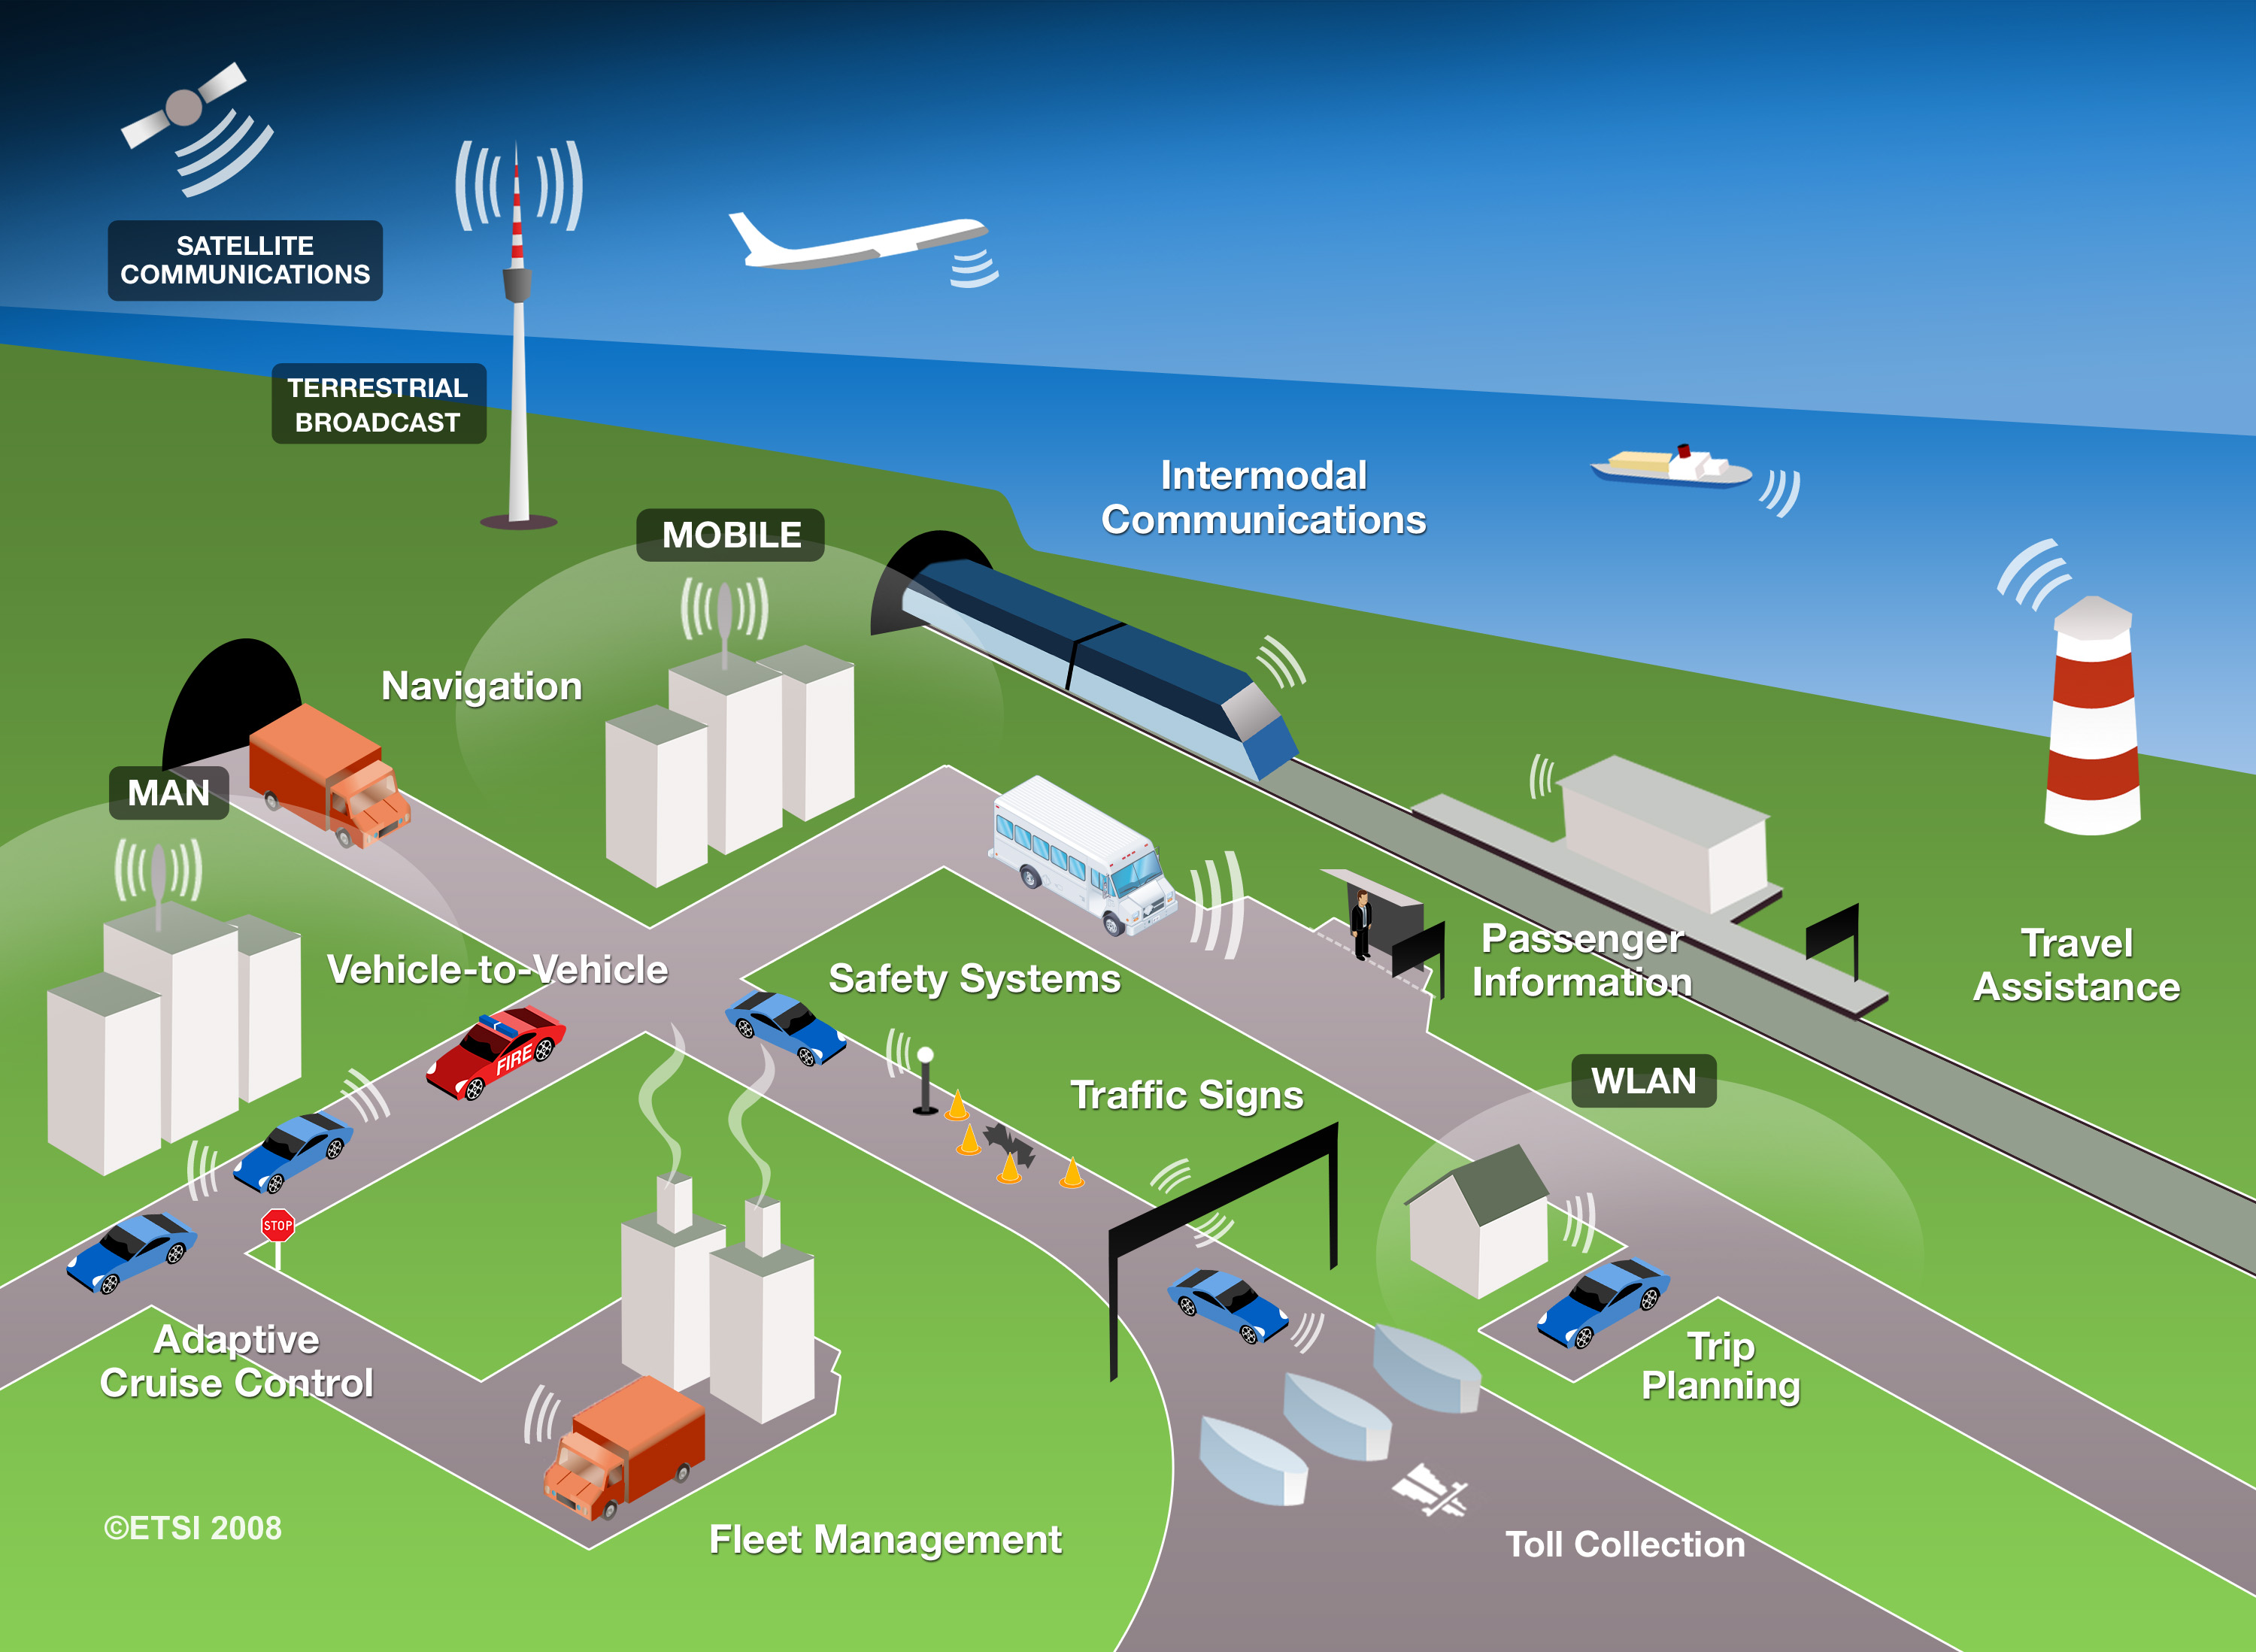
\includegraphics[height=0.8\textheight]{figuras/ITS.png}
    \caption{Aplicaciones en un ITS (fuente: ETSI \autocite{etsi})}
    \label{fig:itsetsi}
\end{figure}
\end{frame}

\begin{frame}{Motivación y Marco Teórico}
Factor común: recopilación y transmisión de información.

Realizado a través de la integración de comunicación inalámbrica en el sistema: LTE, 802.11p (WAVE), etc (\autocite{80211dailey,80211wave,80215vanet,dar2010wireless})
\end{frame}

\begin{frame}{Motivación y Marco Teórico}
\textbf{Problemática:} la tecnología aún está en su infancia, y existen consecuencias de esta integración que deben estudiarse antes de una implementación a gran escala \autocite{sommer2008need}:
\begin{itemize}
    \item efectos de la comunicación sobre el modelo de transporte;
    \item efectos de la topología de la red sobre las comunicaciones.
\end{itemize}
\end{frame}


\begin{frame}{Estado del Arte}
\end{frame}
    
\section{Especificación del Problema}
\section{Diseño e Implementación}
\section{Validación}
\section{Conclusiones}
\begin{frame}[standout]
Thank you!
\end{frame}

\begin{frame}[t,allowframebreaks]{Referencias}
\printbibliography[heading=none]
\end{frame}

\end{document}